% Copyright 2026 Sreeram Anil
% SPDX-License-Identifier: CC-BY-4.0
% =============================================================================
%  Square-root cubature Kalman filter — classical Kalman family
% =============================================================================
\chapter{Square-Root Cubature Kalman Filter (SCKF)}
\label{ch:sckf}

\section*{At a glance}
\begin{tabular}{@{}l>{\raggedright\arraybackslash}p{0.76\textwidth}@{}}
Family & classical Kalman (sigma-point, factored) \\
Header & \texttt{include/estkit/filters/sckf.hpp} \\
Registered name & \texttt{SCKF} \\
State dimension & $n_x = 4$ (cell model) --- generic in $n_x, n_u, n_y$ \\
Propagated quantity & $\mS$ with $\mP = \mS\mS^\T$ (lower triangular) \\
Cost per step & $\mathcal{O}(n_x^3)$ (two QRs) plus $4n_x$ model calls; $1.49$--$1.62\,\SI{}{\micro\second}$/step \\
Primary references & \cite{arasaratnam2009ckf,kailath2000,kaminski1971,golubvanloan2013} \\
\end{tabular}

\section{Motivation and aerospace/BMS relevance}
A covariance filter subtracts: $\Pplus = \Pminus - \mW\mP_{zz}\mW^\T$. When the measurement
is much more informative than the prior, the two terms nearly cancel and the result loses
significant digits; if enough are lost, $\Pplus$ becomes indefinite, the next Cholesky
factorisation fails and the filter diverges. This was the dominant practical failure mode of
Kalman filters in the 1960s and it is what motivated the entire square-root
literature~\cite{kaminski1971}.

A square-root filter never forms $\mP$. It propagates a factor $\mS$ with $\mP = \mS\mS^\T$
through orthogonal transformations, so $\mP$ is positive semi-definite by construction and
the quantity actually stored has condition number $\sqrt{\kappa(\mP)}$ instead of
$\kappa(\mP)$ --- equivalently, the filter behaves like a covariance filter running with
twice the mantissa length. For a battery management unit built on a single-precision
Cortex-M4F, where $\varepsilon \approx 1.2\times10^{-7}$, this is the difference between a
filter that is provably safe and one that has to be argued about: on the eVTOL mission the
peak condition number of $\mP$ is $1.3\times 10^6$, i.e. $\kappa\varepsilon \approx 0.16$ for
the covariance form and $1.4\times10^{-4}$ for the square-root form.

Section~VI of Arasaratnam and Haykin~\cite{arasaratnam2009ckf} gives the square-root form of
the cubature filter; this chapter implements it and verifies that it reproduces the
covariance CKF of Chapter~\ref{ch:ckf} to machine precision.

\section{Problem statement and assumptions}
Model \eqref{eq:ekf-proc}--\eqref{eq:ekf-meas} with additive noise, exactly as the CKF. In
addition it is assumed that Cholesky factors of $\mQ$ and $\mR$ are available (they are
computed once per step by \code{cholesky\_safe}), and that $n_y \le n_x$ so that the
pre-arrays are well shaped --- neither is restrictive.

\section{Derivation}
\paragraph{The triangularisation operator.} For $\mA\in\real^{n\times m}$ with $m\ge n$
define
\begin{equation}
\operatorname{Tria}(\mA) := \mR_{\mathrm{qr}}^\T, \qquad \text{where } \mA^\T = \mQ_{\mathrm{qr}}\mR_{\mathrm{qr}}
\label{eq:sckf-tria}
\end{equation}
is a QR factorisation of the $m\times n$ matrix $\mA^\T$ with $\mR_{\mathrm{qr}}$ upper
triangular. Then $\operatorname{Tria}(\mA)$ is lower triangular and, because
$\mQ_{\mathrm{qr}}^\T\mQ_{\mathrm{qr}} = \mI$,
\begin{equation}
\operatorname{Tria}(\mA)\operatorname{Tria}(\mA)^\T = \mR_{\mathrm{qr}}^\T\mR_{\mathrm{qr}}
 = \mA\mA^\T .
\label{eq:sckf-tria-prop}
\end{equation}
Equation \eqref{eq:sckf-tria-prop} is the whole trick: every covariance sum of the form
$\sum_j \mB_j\mB_j^\T$ is a single matrix product $\mA\mA^\T$ with
$\mA = [\mB_1\;\mB_2\;\cdots]$, so its Cholesky factor is obtained from one orthogonal
triangularisation of the \emph{pre-array} $\mA$ --- the ``array algorithm'' of Kailath, Sayed
and Hassibi~\cite[Ch.~12]{kailath2000}. \code{estkit} implements it with Householder
reflections~\cite[Alg.~5.2.1]{golubvanloan2013} and fixes the sign of the diagonal so that the
factor is unique.

\paragraph{Time update.} Write the weighted, centred propagated points as the columns of
\begin{equation}
\bm{\chi}^* = \frac{1}{\sqrt{m}}\left[\;\mathcal{X}^*_1-\xminus_k \;\;\cdots\;\; \mathcal{X}^*_m-\xminus_k\;\right]
 \in \real^{n_x\times m}, \qquad m = 2n_x .
\label{eq:sckf-chi}
\end{equation}
Then $\bm{\chi}^*\bm{\chi}^{*\T}$ is exactly the sample covariance in \eqref{eq:ckf-tu2}, so
with $\mQ = \mS_Q\mS_Q^\T$
\begin{equation}
\Pminus_k = \bm{\chi}^*\bm{\chi}^{*\T} + \mS_Q\mS_Q^\T
 = \left[\bm{\chi}^*\;\; \mS_Q\right]\left[\bm{\chi}^*\;\; \mS_Q\right]^\T
 \;\Longrightarrow\;
 \mS^-_k = \operatorname{Tria}\!\left(\left[\bm{\chi}^*\;\;\mS_Q\right]\right).
\label{eq:sckf-tu}
\end{equation}
The pre-array is $n_x\times(m+n_x) = 4\times 12$.

\paragraph{Measurement update.} With $\mathcal{Z}_i = h(\mathcal{X}_i,\vu_k)$ and
$\yhat_k$ their mean, define the weighted centred arrays
$\bm{Z}\in\real^{n_y\times m}$ and $\bm{\chi}\in\real^{n_x\times m}$ as in \eqref{eq:sckf-chi}.
Then
\begin{align}
\mS_{zz} &= \operatorname{Tria}\!\left(\left[\bm{Z}\;\;\mS_R\right]\right), &
\mP_{zz} &= \mS_{zz}\mS_{zz}^\T = \bm{Z}\bm{Z}^\T + \mR, \label{eq:sckf-szz}\\
\mP_{xz} &= \bm{\chi}\bm{Z}^\T, &
\mW_k &= \left(\mP_{xz}\mS_{zz}^{-\T}\right)\mS_{zz}\inv, \label{eq:sckf-gain}
\end{align}
the gain being obtained by two triangular back-substitutions rather than by inverting
$\mP_{zz}$. The posterior factor follows from
\begin{equation}
\Pplus_k = \Pminus_k - \mW_k\mP_{zz}\mW_k^\T
 = \left(\bm{\chi}-\mW_k\bm{Z}\right)\left(\bm{\chi}-\mW_k\bm{Z}\right)^\T + \left(\mW_k\mS_R\right)\left(\mW_k\mS_R\right)^\T,
\label{eq:sckf-post}
\end{equation}
which is verified by expanding the right-hand side, using $\bm{\chi}\bm{\chi}^\T=\Pminus_k$,
$\bm{\chi}\bm{Z}^\T = \mP_{xz}$ and $\mW_k\mP_{zz}\mW_k^\T = \mW_k\mP_{xz}^\T = \mP_{xz}\mW_k^\T$.
Hence
\begin{equation}
\mS^+_k = \operatorname{Tria}\!\left(\left[\;\bm{\chi}-\mW_k\bm{Z} \;\;\; \mW_k\mS_R\;\right]\right),
\label{eq:sckf-sp}
\end{equation}
a $n_x\times(m+n_y) = 4\times 9$ pre-array. Note that \eqref{eq:sckf-post} is a \emph{sum} of
two positive semi-definite terms: the subtraction that endangers the covariance form has
disappeared.

\section{Algorithm}
\begin{algorithm}[H]
\caption{SCKF --- one sampling period (additive noise)}
\begin{algorithmic}[1]
\Require $\xplus_{k-1},\mS^+_{k-1},\vu_{k-1},\vy_k,\vu_k$
\State $\mathcal{X}_{i},\mathcal{X}_{i+n_x}\gets\xplus_{k-1}\pm\sqrt{n_x}\,(\mS^+_{k-1})_{:,i}$
\State $\mathcal{X}_i \gets f(\mathcal{X}_i,\vu_{k-1})$;\; $\xminus_k\gets\frac{1}{m}\sum_i\mathcal{X}_i$
\State $\bm{\chi}^*\gets m^{-1/2}[\mathcal{X}_i-\xminus_k]_i$;\; $\mS_Q\gets\operatorname{chol}(\mQ)$
\State $\mS^-_k\gets\operatorname{Tria}([\bm{\chi}^*\;\;\mS_Q])$
\State \textbf{Regenerate} $\mathcal{X}_i$ from $(\xminus_k,\mS^-_k)$;\;
       $\mathcal{Z}_i\gets h(\mathcal{X}_i,\vu_k)$;\; $\yhat_k\gets\frac1m\sum_i\mathcal{Z}_i$
\State $\bm{Z}\gets m^{-1/2}[\mathcal{Z}_i-\yhat_k]_i$;\; $\bm{\chi}\gets m^{-1/2}[\mathcal{X}_i-\xminus_k]_i$;\;
       $\mS_R\gets\operatorname{chol}(\mR)$
\State $\mS_{zz}\gets\operatorname{Tria}([\bm{Z}\;\;\mS_R])$;\; $\mP_{xz}\gets\bm{\chi}\bm{Z}^\T$
\State $\mW\gets(\mP_{xz}/\mS_{zz}^\T)/\mS_{zz}$ \Comment{two triangular solves}
\State $\xplus_k\gets\xminus_k+\mW(\vy_k-\yhat_k)$;\;
       $\mS^+_k\gets\operatorname{Tria}([\bm{\chi}-\mW\bm{Z}\;\;\;\mW\mS_R])$
\State \textbf{if} constraints enabled \textbf{then} $\xplus_k\gets\Pi(\xplus_k)$
\Ensure $\xplus_k,\mS^+_k$ \quad ($\mP$ reconstructed on demand as $\mS^+\mS^{+\T}$)
\end{algorithmic}
\end{algorithm}

\section{Application to the battery model}
The algorithm is identical to the CKF's; only the arithmetic differs. For the cell model the
pre-arrays are $4\times12$ (time update), $1\times9$ ($\mS_{zz}$) and $4\times9$ (posterior),
so the two Householder passes cost $\approx 2(m+n_x)n_x^2 \approx 400$ multiply-accumulates
per step --- about $26\,\%$ more than the covariance CKF, which matches the measured
$1.49$--$1.62\,\SI{}{\micro\second}$ against $1.18$--$1.26\,\SI{}{\micro\second}$.

The benchmark adapter reads $\sigma_\soc$ from $\mP$ to report a confidence band, so the
filter exposes $\mP$ through a cached reconstruction $\mS\mS^\T$ that is recomputed only when
$\mS$ has changed (one $4\times4$ product, and only when the accessor is actually called).

\section{Implementation notes}
\code{kalman\_detail::tria} is a three-line wrapper around \code{qr\_r}, which is the one
piece of numerical machinery this filter needs. The sign convention in \code{qr\_r} (diagonal
made non-negative) guarantees a unique factor, so repeated calls are reproducible bit for
bit. \code{cholesky\_safe} is used for $\mQ$ and $\mR$; it adds diagonal jitter on failure, so
a numerically semi-definite $\mQ$ cannot abort the step. Guard: if the gain is not finite the
update is skipped and the prior kept. Memory: 4696\,bytes, of which the filter state proper is
$\mS$ ($16$ reals), $\vx$ ($4$) and the cached $\mP$ ($16$).

Verification: run against the covariance CKF over a full nominal mission
($\num{18000}$ steps), the two agree to $\max\abs{\Delta\vx} = 1.0\times10^{-12}$ and
$\max\abs{\Delta\mP} = 4.8\times10^{-14}$ --- consistent with round-off in double precision
and a direct confirmation of \eqref{eq:sckf-tu}--\eqref{eq:sckf-sp}.

\section{Benchmark results}
% Copyright 2026 Sreeram Anil
% SPDX-License-Identifier: CC-BY-4.0
\begin{table}[H]\centering\footnotesize\setlength{\tabcolsep}{4pt}
\caption{SCKF: cell-level benchmark on the eVTOL mission (mean over seeds; RMSE and max error in \% SOC; $t_\mathrm{conv}$: first time the error stays below 2\,\% for 60\,s, -- = never; EKF reference: steady-state RMSE of the plain EKF on the same data).}\label{tab:cell_SCKF}
\begin{tabular}{llrrrrrcrr}\toprule
plant & scenario & RMSE & RMSE$_\mathrm{ss}$ & max & $t_\mathrm{conv}$ [s] & RMSE$_v$ [mV] & div. & EKF ref. & ns/step \\ \midrule
ECM & nominal & 0.08 & 0.05 & 1.23 & 0 & 0.80 & no & 0.05 & 1581 \\
ECM & init\_error & 1.64 & 0.09 & 6.63 & 221 & 2.11 & no & 0.05 & 1581 \\
ECM & current\_bias & 0.48 & 0.55 & 1.19 & 0 & 0.87 & no & 0.61 & 1616 \\
ECM & noise\_step & 0.14 & 0.15 & 1.23 & 0 & 2.89 & no & 0.12 & 1577 \\
ECM & outliers & 0.35 & 0.07 & 4.54 & 4 & 2.08 & no & 0.21 & 1579 \\
ECM & cold & 0.15 & 0.11 & 1.12 & 0 & 1.90 & no & 0.16 & 1574 \\
ECM & hot & 0.08 & 0.04 & 1.27 & 0 & 0.56 & no & 0.03 & 1580 \\
ECM & aged\_cell & 2.87 & 1.79 & 9.21 & 0 & 3.78 & no & 1.52 & 1574 \\
ECM & param\_mismatch & 1.56 & 1.59 & 3.92 & 0 & 2.83 & no & 1.36 & 1573 \\
ECM & sensor\_dropout & 2.83 & 1.92 & 7.59 & 0 & 1.86 & no & 0.46 & 1567 \\
ECM & preisach & 1.20 & 0.24 & 4.25 & 218 & 0.84 & no & 0.20 & 1581 \\
ECM & combined & 13.07 & 11.26 & 23.22 & -- & 4.88 & no & 12.44 & 1589 \\
\midrule
SPM & nominal & 4.72 & 4.62 & 6.18 & 0 & 1.03 & no & 3.73 & 1510 \\
SPM & init\_error & 5.17 & 4.69 & 6.70 & -- & 2.17 & no & 3.81 & 1499 \\
SPM & current\_bias & 6.07 & 6.65 & 7.49 & 0 & 1.12 & no & 5.69 & 1507 \\
SPM & noise\_step & 4.26 & 3.77 & 6.18 & 0 & 3.14 & no & 3.30 & 1527 \\
SPM & outliers & 2.21 & 2.21 & 4.40 & 0 & 2.32 & no & 1.99 & 1498 \\
SPM & cold & 8.61 & 8.72 & 11.29 & -- & 4.04 & no & 7.35 & 1500 \\
SPM & hot & 2.74 & 2.73 & 3.40 & 0 & 0.70 & no & 2.16 & 1504 \\
SPM & param\_mismatch & 4.56 & 4.81 & 5.52 & 0 & 1.97 & no & 3.13 & 1493 \\
SPM & sensor\_dropout & 8.12 & 8.24 & 9.78 & 0 & 1.92 & no & 5.31 & 1502 \\
\bottomrule\end{tabular}\end{table}

\begin{figure}[H]\centering
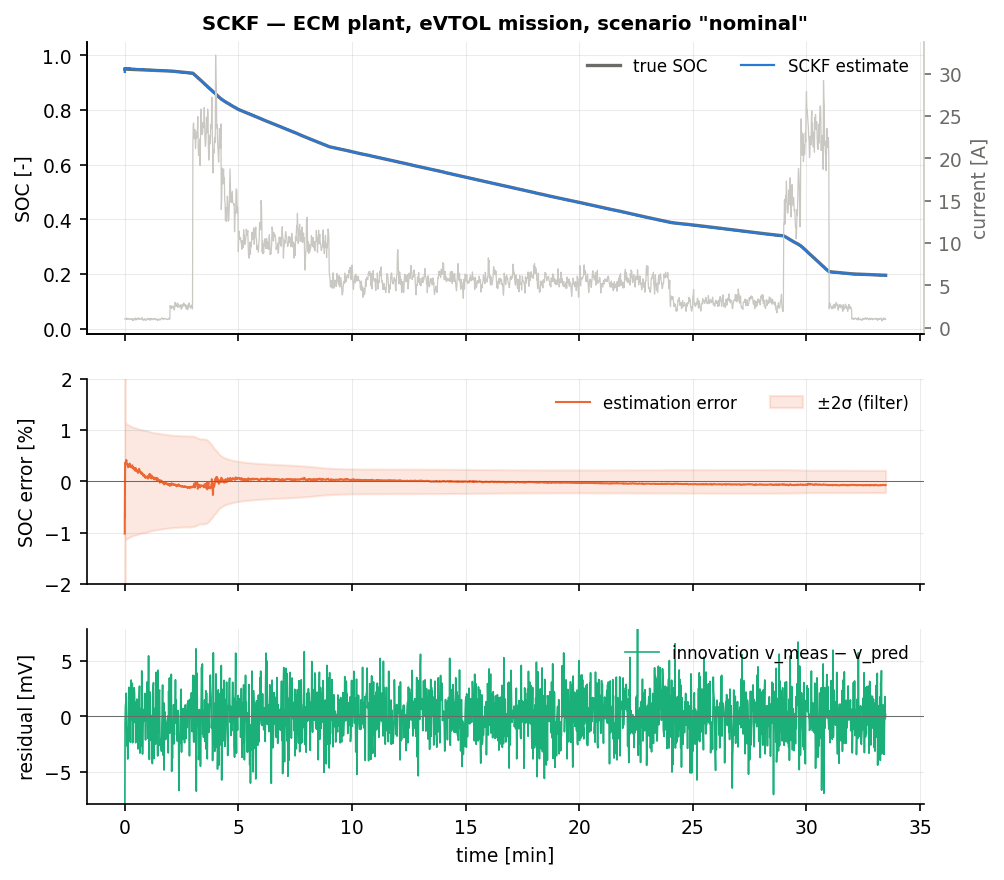
\includegraphics[width=\textwidth]{figures/cell_SCKF_nominal.png}
\caption{SCKF on the nominal eVTOL mission: true and estimated SOC (top), estimation error with the $\pm 2\sigma$ band when available (middle), voltage residual (bottom).}
\end{figure}
\begin{figure}[H]\centering
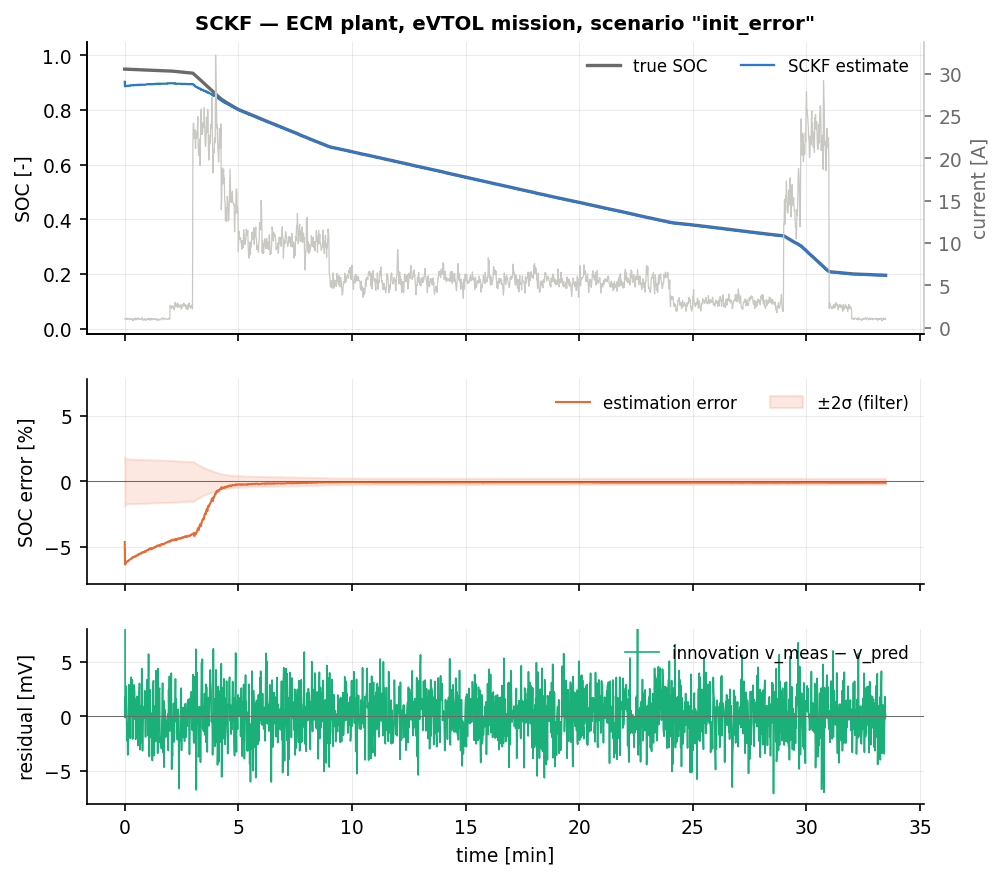
\includegraphics[width=\textwidth]{figures/cell_SCKF_init_error.png}
\caption{SCKF with a 35\,\% initial SOC error.}
\end{figure}

All numbers are three-seed means in per cent SOC.

The SCKF reproduces the CKF on every scenario of both plants to the two decimals printed by the
table: ECM \texttt{nominal} $0.08/0.05\,\%$, \texttt{init\_error} $1.64/0.09\,\%$ with
$t_{\text{conv}} = 221$\,s, \texttt{outliers} $0.35/0.07\,\%$, \texttt{aged\_cell}
$2.87/1.79\,\%$, \texttt{sensor\_dropout} $2.83/1.92\,\%$, \texttt{combined}
$13.07/11.26\,\%$; SPM \texttt{nominal} $4.72/4.62\,\%$, \texttt{cold} $8.72\,\%$. That is the
expected and desired result --- a square-root filter is not a different estimator, it is the
same estimator in different arithmetic --- and the discussion of Chapter~\ref{ch:ckf} applies
verbatim, including the slow convergence from a wide prior and the failure on
\texttt{combined}.

The interesting question is what the factorisation buys. On this problem, in double precision,
nothing measurable: the covariance form never lost definiteness. The float-versus-double table
confirms it in single precision as well --- both forms give $0.05\,\%$ on \texttt{nominal} and
$0.09\,\%$ on \texttt{init\_error} in float32, and on \texttt{aged\_cell} the square-root form
is marginally better ($2.48\,\%$ against $2.53\,\%$) --- which says that $n_x = 4$ with
$\kappa(\mP)\le1.3\times10^6$ is simply not a hard enough problem to separate them. The honest
conclusion is that the square-root form is insurance rather than an improvement: it costs
$26\,\%$ more time ($1.49$--$1.62\,\SI{}{\micro\second}$ against $1.18$--$1.26$) and removes an
entire class of failure that this particular benchmark does not exercise. The situations where
it does matter are well documented~\cite{verhaegen1986}: larger state dimension,
near-deterministic states (very small $\mQ$ entries, as in parameter augmentation), very
accurate sensors (small $\mR$), or fixed-point arithmetic.

The one genuinely different number is the runtime, and it is worth noting that the SCKF's cost
is almost entirely deterministic: two Householder passes of fixed size, no conditional
branches, no matrix inversion. For a hard-real-time BMS task that predictability can be worth
more than the $300$\,ns.

\paragraph{SPM plant: structured model error.}
\begin{figure}[H]\centering
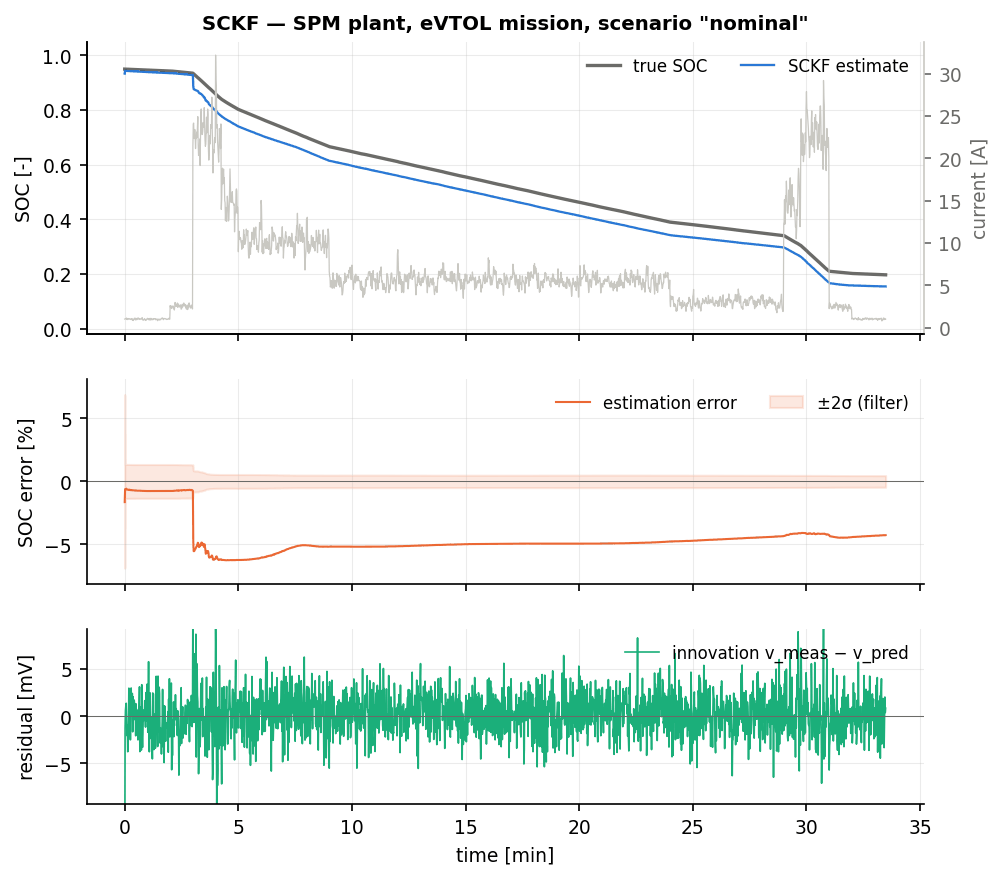
\includegraphics[width=\textwidth]{figures/cellspm_SCKF_nominal.png}
\caption{SCKF on the nominal mission with the electrochemical (SPM) plant; identical to the covariance CKF.}
\end{figure}
The SPM block of the table is a different kind of test. The plant is the electrochemical
single-particle model; the estimator still runs a 2-RC equivalent circuit, fitted to that plant,
which leaves a \emph{structured} residual of about $4$\,mV (Butler--Volmer kinetics and
solid-phase diffusion that no 2-RC circuit can reproduce) and a slow second branch,
$\tau_2 = 556$\,s. Over a $33$-minute mission a $556$\,s pole barely relaxes, so $v_2(t)$ is
close to an affine ramp --- and so is $\ocv(\soc(t))$ while the cell discharges at a roughly
constant rate. The two channels through which the measurement sees the state,
$(\partial\ocv/\partial\soc)\,\delta\soc$ and $-\delta v_2$, are therefore nearly collinear in
the information accumulated over the flight: the pair $(\soc, v_2)$ is close to unobservable,
and no filter can decide whether a persistent few-millivolt residual belongs to the slow RC
branch or to the state of charge. Because that direction is weakly observable, a $4$\,mV
structured error maps onto \emph{several per cent} of SOC instead of the
$4\,\text{mV}/0.8\,\text{V}\approx0.5\,\%$ a well-conditioned channel would give. This
$(\soc,v_2)$ ambiguity, not the size of the residual, is the mechanism behind the
$3.7$--$4.6\,\%$ band in which the whole classical family sits.

The cubature filters are the \emph{worst} of the family here: $4.62\,\%$ on SPM
\texttt{nominal} against the EKF's $3.73\,\%$ and the LKF's $1.72\,\%$, $8.72\,\%$ on
\texttt{cold} against $7.35\,\%$, $8.24\,\%$ on \texttt{sensor\_dropout} against $5.31\,\%$ and
$4.81\,\%$ on \texttt{param\_mismatch} against $3.13\,\%$. The ordering across the whole family
is in fact monotone in the sigma-point spread --- LKF (frozen tangent) $1.72$, EKF/IEKF
(tangent at the mean) $3.66$--$3.73$, UKF ($0.2\sigma$ points) $3.96$, cubature filters
($2\sigma$ or $2.45\sigma$ points) $4.61$--$4.62$ --- and the ambiguity argument explains it.
A statistical linearisation taken over a wide prior returns the \emph{chord} of the OCV curve,
which is steeper than the tangent over most of the mission, so the filter believes the OCV
channel is more informative than it is and commits harder to the direction that carries the
structured error. The single exception is \texttt{outliers} ($2.21\,\%$), where every filter
does better on SPM than on ECM because the corrupted samples widen the effective innovation
covariance. Nothing diverges and $t_{\text{conv}} = 0$ on every SPM row: the error is a bias,
not a drift.

The SCKF's SPM rows are identical to the CKF's to two decimals, as they are on the ECM plant.
Worth noting for a square-root chapter: the SPM rows are the only ones in this report where the
filters are visibly \emph{mis-specified}, and even there the covariance form remained positive
definite throughout, so the factorisation again changed nothing. A structurally wrong model
stresses the estimator statistically, not numerically.

\section{Summary}
Use the SCKF whenever a cubature filter has to run in single precision, in fixed point, or on a
problem where $\mP$ can become ill-conditioned (parameter augmentation, very accurate sensors,
large $n_x$); it gives exactly the CKF's estimates with a covariance that cannot go indefinite
and with a deterministic instruction count. On the cell model in double precision it is a
$26\,\%$ tax for insurance you do not need. Its estimation behaviour --- excellent nominal
accuracy, slow convergence from a wide prior, worst of the family under structured model error
--- is that of the CKF, and is discussed in Chapter~\ref{ch:ckf}.
